\documentclass[output=paper]{langscibook} 

\author{Katalin É. Kiss\affiliation{Research Institute for Linguistics} and Lilla Pintér\affiliation{Pázmány Péter Catholic University, Research Institute for Linguistics} and  Tamás Zétényi\affiliation{Budapest University of Technology and Economics}}
\title[Group-denoting vs. counting]{Group-denoting vs. counting: Against the scalar explanation of children's interpretation of `some'}  
\abstract{The computation of scalar implicatures based on the scale $\stb{\textit{some, all}}$ represents a problem for children. This paper argues that the source of children’s difficulties with interpreting `some' is that it is ambiguous; it has a non-partitive interpretation, corresponding to `a few', which forms a scale with non-partitive `many', and a partitive reading, corresponding to `a subset of', which forms a scale with `all'. The two readings have different distributions; they are selected by different predicates, and in Hungarian, they occur in different structural positions. We tested and confirmed the hypothesis that young children are not sensitive to the partitivity feature of `some'-phrases; they first acquire the non-partitive reading, which they overgeneralize for a while. Experiment 1, a forced choice task, showed that the default reading of `some' NPs for six-year olds is the `a few' interpretation. Experiment 2, a truth value judgement task, demonstrated that children also accept the `not all' interpretation of `some', and the acceptance rates of the `a few' and the `not all' readings are similar irrespective of the partitivity feature of the given NP.

\keywords{scalar implicature, `some', counting quantifier, partitive, Hungarian, language acquisition}}

\begin{document}
\maketitle


\section{Introduction}\label{kis-zet:sec:introduction}

Whereas adults interpret \textit{some} e.g. in  \textit{Some horses jumped over the fence} as `some but not all', children understand it as `some and possibly all' \citep[e.g.][]{noveck2001children,papafragou2004children}. It has been claimed that the basic meaning of plural \textit{some} is `some and possibly all', and the `some but not all' reading is a pragmatic inference, a scalar implicature, which children cannot access \citep[see][]{noveck2001children,chierchia2001acquisition,papafragou2003scalar,guasti2005children,foppolo2012scalar,huang2009online,katsos2011pragmatic,barner2011accessing}. The assumption that children generally have problems with computing scalar implicatures cannot explain though why pragmatic inferencing has proved to be much easier for them in the case of scales involving cardinal numbers than in the case of the scale involving \textit{some} and \textit{all} \citep{papafragou2003scalar}.

Recently it has been proposed that a scalar implicature is often a problem for children because they lack knowledge of the relevant scalar alternatives. That is, young children accept \textit{some} in situations which could be more appropriately described by \textit{all} because they are still not aware of the fact that \textit{all} is a stronger alternative of the same scale that includes \textit{some} \citep{barner2011accessing,foppolo2012scalar,pagliarini2018children}.

We argue that the source of children's difficulties with interpreting \textit{some} and its Hungarian equivalent \textit{néhány} is that \textit{some/néhány} is ambiguous. It has a non-partitive interpretation, corresponding to `a few', which forms a scale with non-partitive \textit{many}, and a partitive reading, corresponding to `a subset of', which forms a scale with \textit{all}.\footnote{\textit{Many} also has a non-partitive reading, paraphraseable as `a large number of', and a partitive or proportional reading, paraphraseable as `a large subsection of'. This well-known ambiguity is discussed in connection with examples \REF{kis-zet:nehany vendeg a}--\REF{kis-zet:nehany vendeg b}, \REF{kis-zet:blossom}--\REF{kis-zet:some films}, and \REF{kis-zet:some major mistakes}--\REF{kis-zet:some mistakes}.} The two variants of \textit{some/néhány} have different distributions; they are selected by different predicates, and in Hungarian, they occur in different structural positions. We have hypothesized that for young children, the primary reading of `some' NPs is the non-partitive reading; this is what explains their behaviour in the experiments cited above. We tested this assumption with the two experiments to be presented in this paper.

The paper is organized as follows: \sectref{kis-zet:sec:group-vs-count} presents linguistic evidence of the ambiguity of \textit{néhány}  `some'. \sectref{kis-zet:sec:acquisition} surveys previous experiments testing children's interpretation of `some'. \sectref{kis-zet:sec:experiments} presents our own experiments with \textit{néhány}. \sectref{kis-zet:sec:conclusion} is the conclusion.

\section{Group-denoting versus counting \textit{néhány/some}: Linguistic evidence}\label{kis-zet:sec:group-vs-count}

For adults, a \textit{some} NP in English or a \textit{néhány}  NP in Hungarian is often ambiguous, e.g.:

\ea
\gll Találkoztam néhány diákkal.\\  
     meet.\textsc{past}.\textsc{1sg} some student.with\\ 
\glt `I met some students.'\label{kis-zet:ex:nehany}
\z

\noindent The Hungarian sentence and its English equivalent in \REF{kis-zet:ex:nehany} can mean both that I met a small indefinite number of students, and that I met a (small) subset of a contextually given set of students. (To what extent the `small' component is part of the latter, partitive meaning, as well, appears to be individual dependent – as was revealed by the reactions of the adult control group of our experiments. In the experiments of \citet{degen2015processing}, the default set size associated with \textit{some} by English adults is 6--8.)

In two structural positions in the functional left periphery of the Hungarian sentence, the \textit{néhány} phrase ceases to be ambiguous. These are the two preverbal slots of the basic Hungarian sentence: a topic slot (the specifier of an iterable TopP), accessible to referential constituents, and an immediately preverbal slot (the specifier of PredP) harboring a non-referential, predicative complement – as shown in \figref{kis-zet:tree} (for details, see \citealt{ekiss2002syntax,ekiss08,ekiss10,szabolcsi1994notequal,szabolcsi1997strategies}, among others).

\begin{figure}
    \centering
    \begin{forest}
    for tree={s sep=1cm, inner sep=0cm, l=0cm}
    [TopP
        [Spec, name=topic
            [topic]
        ]
        [PredP
            [Spec
                [predicative complement] 
            ]
            [Pred$'$
                [Pred
                    [V, name=V]
                ]   
                    [VP
                            [{{} {} {} {} {} t\textsubscript{V} {} {} {} {} {}}, roof]
                   ]     
                ]
            ]
        ]
    \end{forest}
    \caption{Hungarian sentence structure}
    \label{kis-zet:tree}
\end{figure}

\noindent The topic and the filler of SpecPredP can be separated by sentence adverbials, by distributive quantifiers, and by an exhaustive focus. The topic precedes the (first) pitch accent, whereas the constituent in SpecPredP either itself bears a pitch accent, or follows another pitch-accent-bearing element.

In the topic position, the \textit{néhány} phrase is understood to denote a (small) subset of a contextually given set – see examples \REF{kis-zet:ex:nehany diakkal a} and \REF{kis-zet:ex:nehany diakkal b}, where the topic status of the \textit{néhány} phrase is ensured by its position preceding the universal quantifier, the locus of pitch accent (denoted by ʹ). \REF{kis-zet:ex:nehany diakkal a} and \REF{kis-zet:ex:nehany diakkal b} represent the same structure, with the grammatical functions distributed in different ways; they illustrate that word order in the preverbal section of the Hungarian sentence is determined by logical role rather than grammatical functions.

\eal\label{kis-zet:ex:nehany diakkal}
\ex[]{
\gll [\textsubscript{TopP} Néhány diák	[$_\text{DistP}$ \minsp{ʹ} minden	professzorral\hspace{2cm} 	[$_\text{PredP}$ konzultált.]]]\\
{} some student {} {} every professor.with {} consult.\textsc{past.3sg}\\
\glt `Some students consulted with every professor.'\label{kis-zet:ex:nehany diakkal a}
}
\ex[]{
\gll [$_\text{TopP}$ Néhány diákkal 	[$_\text{DistP}$ \minsp{ʹ} minden	professzor\hspace{2cm} 	[$_\text{PredP}$ konzultált.]]]\\
{} some student.with {} {} every professor {} consult.\textsc{past.3sg}\\
\glt `With some students, every professor consulted.'\label{kis-zet:ex:nehany diakkal b}
}
\zl

\noindent The topic of the sentence represents the logical subject of predication, therefore, it must have restricted reference, i.e., must be specific. Partitivity corresponds to a type of specificity \citep{encc1991semantics,farkas2002specificity,kamp2019epistemic}, thus the partitive interpretation associated with \textit{néhány} in topic position is a manifestation of its specificity feature.

In the specifier of the PredP projection, by contrast, the non-partitive interpretation of \textit{néhány}, corresponding to `a few', is evoked (see \REF{kis-zet:nehany diak erkezett}).  SpecPredP is filled by the non-referential complement of the verb, and its filler has the smallest possible scope \citep{szabolcsi1983specifikus}, which is also true of the \textit{néhány}-phrase in SpecPredP (see \REF{kis-zet:mindharom professzor}). As opposed to the topicalized, partitive \textit{néhány} NP in \REF{kis-zet:ex:nehany diakkal a} and \REF{kis-zet:ex:nehany diakkal b}, the non-partitive \textit{néhány} NP in SpecPredP bears a pitch accent. The relative stress of \textit{néhány} within the NP is also different in the two cases: whereas the partitive \textit{néhány}, a strong determiner, itself bears the secondary stress of the \textit{néhány} NP, in the non-partitive \textit{néhány} NP, the pitch accent falls on the nominal determined by \textit{néhány}.

\eal
\ex[]{
\gll [$_\text{PredP}$  Néhány \minsp{ʹ} diák érkezett.]\\
{} some {} student arrive.\textsc{past.3sg}\\
\glt `Some students arrived.'\label{kis-zet:nehany diak erkezett}
}
\ex[]{
\gll [[$_\text{DistP}$ \minsp{ʹ} Mind-három professzor	[$_\text{PredP}$ néhány \minsp{ʹ} diákkal konzultál.]]\\
{} {} all-three professor	{} some {} student.with consults\\
\glt `Each of the three professors is consulting with some students.' \label{kis-zet:mindharom professzor}
}
\zl

\noindent The left periphery of the Hungarian sentence can also include a focus slot between PredP and TopP, in the specifier of a focus phrase (FocP). The focus elicits verb movement from Pred to Foc, hence a preverbal \textit{néhány} NP can sit either in SpecPredP or in SpecFocP. (SpecFocP position is traditionally marked by small capitals.) Whereas the \textit{néhány} NP in SpecPredP is [$-$partitive], the exhaustive/ contrastive \textit{néhány} phrase in SpecFocP is [$\pm$parti\-tive], i.e., it can either mean `a few, not many', or it can mean ‘a (small) subset of a contextually given set, not the whole set’ -- see \textit{néhány diák} `some students' in \REF{kis-zet:csak néhány diákkal}. The excluded alternative shares the partitivity feature of the \textit{néhány} phrase. When \textit{néhány diák} `some students' is understood as [$-$partitive], the excluded alternative is the [$-$partitive] `many students' – see \REF{kis-zet:nem csak néhány diákkal a}. When it is understood as [$+$partitive], what it excludes is `all students' -- see \REF{kis-zet:nem csak néhány diákkal b}. 

\ea
\gll [$_\text{FocP}$ \minsp{(} Csak) \minsp{ʹ} \textsc{néhány} \textsc{diákkal} konzultáltam$_\text{i}$ [$_\text{PredP}$  \textit{t}$_\text{i}$ \dots]]\\
{} {} only {} some student.with consult.\textsc{past}.\textsc{1sg} \\ 
\glt `It was (only) some students that I consulted with.' \label{kis-zet:csak néhány diákkal}
\z

\eal
\ex[]{
\gll [$_\text{NegP}$ Nem [$_\text{FocP}$ \minsp{(} csak) \minsp{ʹ} \textsc{néhány} \textsc{diákkal}	konzultáltam$_\text{i}$\hspace{1cm} [$_\text{PredP}$ \textit{t}$_\text{i}$ \dots]]] hanem sokkal.\\
{} not {} {} only {} some student.with consult.\textsc{past.1sg} {} {} {} but many.with\\
\glt `I consulted not (only) with some students but with many.'\label{kis-zet:nem csak néhány diákkal a}
}
\ex[]{
\gll [$_\text{NegP}$ Nem [$_\text{FocP}$ \minsp{(} csak) \minsp{ʹ} \textsc{néhány} \textsc{diákkal}  	 konzultáltam$_\text{i}$\hspace{1cm} [$_\text{PredP}$ \textit{t}$_\text{i}$ \dots]]] hanem minddel.\\
{} not {} {} only {} some student.with consult.\textsc{past.1sg} {} {} {} but all.with\\
\glt `I consulted not (only) with some students but with all.' \label{kis-zet:nem csak néhány diákkal b}
}
\zl

\noindent In our experiments, we intended to test the interpretations of \textit{néhány} NPs in SpecTopP and in SpecPredP, where they are not ambiguous; i.e., we excluded focussed \textit{néhány} phrases. Since the verb moves to Pred in neutral clauses, and moves on to Foc in focus constructions, an immediately preverbal \textit{néhány} can, in principle, occupy either SpecPredP or SpecFocP; however, the filler of SpecFocP and the filler of SpecPredP behave differently under negation, which makes their identity easily testable. Namely, FocP negation elicits no further verb movement, resulting in a Neg–SpecFocP–V order – as shown in \REF{kis-zet:nem csak néhány diákkal a} and \REF{kis-zet:nem csak néhány diákkal b}. PredP negation, on the contrary, elicits V-to-Neg movement, yielding a Neg–V–SpecPredP order \REF{kis-zet:nem érkezett a}; \REF{kis-zet:nem konzultált a}. A non-partitive \textit{néhány} phrase inside a negated PredP is marginal; it tends to be replaced by the negative polarity indefinite \textit{egy\dots sem} `not even one; no' \REF{kis-zet:nem érkezett b}; \REF{kis-zet:nem konzultált b}: 

\eal
\ex[$^\text{?}$]{
\gll [$_\text{NegP}$ \minsp{ʹ} Nem 	érkezett$_\text{i}$  [$_\text{PredP}$ néhány diák \textit{t}$_\text{i}$ \dots]]\\
{} {} not arrive.\textsc{past.3sg} {} some student \\
\glt ‘It is not the case that some students have arrived.’\label{kis-zet:nem érkezett a}
}
\ex[]{
\gll [$_\text{NegP}$ \minsp{ʹ} Nem érkezett$_\text{i}$ [$_\text{PredP}$ egy 	diák 		sem 	\textit{t}$_\text{i}$ \dots]]\\
{} {} not arrive.\textsc{past.3sg} {} one student even\\
\glt `No student arrived.'\label{kis-zet:nem érkezett b}
}
\zl

\eal
\ex[$^\text{?}$]{
\gll [$_\text{TopP}$ A professzor [$_\text{NegP}$ \minsp{ʹ} nem konzultált$_\text{i}$  [$_\text{PredP}$ néhány diákkal \textit{t}$_\text{i}$ \dots]]\\
{} the professor {} {} not consult.\textsc{past.3sg} {} some student.with\\
\glt `It is not the case that the professor consulted with some students.'\label{kis-zet:nem konzultált a}
}
\ex[]{
\gll [$_\text{TopP}$ A professzor [$_\text{NegP}$ \minsp{ʹ} nem konzultált$_\text{i}$  [$_\text{PredP}$ egy diákkal sem \textit{t}$_\text{i}$ \dots]]\\
{} the professor {} {} not consult.\textsc{past.3sg} {} one student.with even\\
\glt `The professor did not consult with any student.'\label{kis-zet:nem konzultált b}
}
\zl

\noindent The claim that the different preverbal positions of the Hungarian sentence let in different types of quantifiers was first made by \citet{szabolcsi1994notequal, szabolcsi1995modes}. She claimed that the topic position is open to group-denoting quantifiers such as \textit{a fiú} `the boy', \textit{hat fiú} `six boys'; the distributive quantifier position is open to universals, among others, whereas the specifier of PredP can take so-called counting quantifiers such as \textit{pontosan hat fiú} `exactly six boys', \textit{kevés fiú} `few boys', \textit{hatnál kevesebb fiú} `less than six boys', \textit{sok fiú} `many boys' etc. The difference between counting and non-counting quantifiers is procedural. The mode of operation of group-denoting (and distributive) quantifiers is ``predicate and +/-distribute'', and that of counting quantifiers is ``count''. Group-denoting and distributive DPs are monotonically increasing quantifiers whose witness sets serve as logical subjects of predication. Their combination with a predicate asserts that the predicate holds, or does not hold, of that witness set or its elements. In contrast, counting quantifiers specify the size of a participant of the atomic or plural event described by the verbal predicate in conjunction with the counting quantifier’s restriction. \citet{szabolcsi2010quant} associates the two interpretations with Brentano’s categorical and thetic judgments, citing \citet{ladusaw1994thetic}.

\citet{szabolcsi1994notequal, szabolcsi1995modes, szabolcsi2010quant} also called attention to the fact that a noun phrase can belong to more than one quantifier type, and its behavior and interpretation in Hungarian depends on which position it occupies in the sentence structure. For example, \textit{sok fiú} `many boys' can stand both in SpecDistP \REF{kis-zet:asztal a} and in SpecPredP \REF{kis-zet:asztal b}, and it is obligatorily distributive only in the distributive quantifier position \REF{kis-zet:asztal a}:

\eal
\ex[]{
\gll [$_\text{DistP}$ \minsp{ʹ} Sok fiú [$_\text{PredP}$ \minsp{ʹ} fel emelte az asztalt.]]\\
{} {} many boy {} {} up lift.\textsc{past.3sg} the table.\textsc{acc}\\
\glt `Many boys each lifted the table.'\label{kis-zet:asztal a}
}
\ex[]{
\gll [$_\text{PredP}$ \minsp{ʹ} Sok fiú emelte$_\text{i}$ [$_\text{vP}$ fel t$_\text{i}$ az asztalt.]]\\
{} {} many boy lift.\textsc{past.3sg} {} up {} the table.\textsc{acc}\\
\glt `Many boys lifted the table.'\label{kis-zet:asztal b}
}
\zl

\noindent When functioning as a non-counting quantifier, \textit{sok} assumes a partitive interpretation; it marks a value of the scale involving `all'. When used as a counting quantifier, it lacks partitivity; it forms a scale with `few', among others. Compare the interpretations of \textit{sok} in SpecDistP and in SpecPredP. While \REF{kis-zet:tüntetes a} is a meaningful statement confronting two large subsets of a contextually given set, \REF{kis-zet:tüntetes b} involves a contradiction, making two opposing statements about an event. 

\eal
\ex[]{
\gll [$_\text{DistP}$ \minsp{ʹ} Sok diák [$_\text{PredP}$ \minsp{ʹ} el jött a tüntetésre]], sok diák \minsp{ʹ} nem jött el.\\
{} {} many student {} {} off come.\textsc{past.3sg} the demontration.to many student {} not come.\textsc{past.3sg} off\\
\glt `Many students have come to the demonstration; many students haven’t come.'\label{kis-zet:tüntetes a}
}
\ex[*]{
\gll [$_\text{PredP}$ \minsp{ʹ} Sok diák jött a tüntetésre], \minsp{ʹ} nem jött sok diák.\\
{} {} many student come.\textsc{past.3sg} the demontration.to {} not come.\textsc{past.3sg} many student\\
\glt Intended: `There arrived many students at the demonstration; there didn’t arrive many students.'\label{kis-zet:tüntetes b}
% \glt *‘There arrived many students at the demonstration; there didn’t arrive many students.’\label{kis-zet:tüntetes b}
}
\zl

\noindent Notice that the \textit{sok} phrase in SpecDistP of the second clause of \REF{kis-zet:tüntetes a} precedes the negative particle and is outside the scope of negation, whereas the \textit{sok} phrase in SpecPredP of the second clause of \REF{kis-zet:tüntetes b} follows the negated verb, and is inside the scope of negation.

The different partitivity features of non-counting and counting quantifiers are manifested in further facts of Hungarian. Hungarian syntactically distinguishes verbs of creation and coming-into-being from their change-of-state counterparts \citep{szabolcsi1986definiteness,pinon08}. Verbs stating the existence, or appearance, or creation of an individual have an obligatorily non-specific, hence non-partitive, internal argument – one whose existence or coming into being is asserted or nega\-ted \REF{kis-zet:vendég a}. Notice that if these verbs take a telicizing verbal particle, they express the change-of-state of an individual that has already existed partially or in the form of a plan, and the noun phrase denoting this individual is obligatorily partitive-specific \REF{kis-zet:vendég b}. (In English, the existence/coming-into-being/creation interpretation and the change-of-state interpretation are not distinguished formally. The \textit{there is} construction enforces the existence/coming-into-being reading, but a ‘preverbal subject, verb’ complex is ambiguous. For a detailed semantic analysis of the two readings, see \citealt{pinon08}.)  

\eal
\ex[]{
\gll \minsp{\{} Vendég / \minsp{*} a  vendég / \minsp{*} Mari vendége / \minsp{*} minden vendég\}	 érkezett.\\
{} guest {} {} the guest {} {} Mary guest.\textsc{3sg} {} {} every guest 	 arrive.\textsc{past.3sg}\\
\glt `There arrived a guest/*the guest/*Mary’s guest/*every guest.'\label{kis-zet:vendég a}
}
\ex[]{
\gll \minsp{\{} A vendég / Mari vendége / minden vendég / \minsp{*} vendég\}	meg érkezett.\\
{} the guest {} Mary guest.\textsc{3sg} {} every guest {} {} guest    	\textsc{prt}  arrive.\textsc{past.3sg}\\
\glt `The guest/Mary’s guest/every guest/*guest arrived.'\label{kis-zet:vendég b}
}
\zl

\noindent The \textit{sok} determiner of a noun phrase complementing a particleless verb of existence, coming-into-being or creation is understood as `a large number of' \REF{kis-zet:sok vendég a}, whereas the \textit{sok} determiner of a phrase complementing a particle verb expressing the change-of-state of a presupposed referent is understood as `a large subset of' \REF{kis-zet:sok vendég b}:

\eal
\ex[]{
\gll Sok vendég érkezett.\\
many guest arrive.\textsc{past.3sg}\\
\glt ‘There arrived a large number of guests.’\label{kis-zet:sok vendég a}
}
\ex[]{
\gll Sok vendég meg érkezett.\\
many guest \textsc{prt}  arrive.\textsc{past.3sg}\\
\glt `A large subset of the guests arrived.'\label{kis-zet:sok vendég b}
}
\zl

\noindent In Hungarian, \textit{néhány} `some' NPs behave similarly to \textit{sok} phrases in that they can occur in different preverbal positions, where they represent different quantifier types. A \textit{néhány} phrase can stand in SpecTopP, where it behaves as a group-denoting quantifier, or it can stand in SpecPredP, where it acts as a counting quantifier. The test demonstrating the interpretive difference of the partitive-specific non-counting use in SpecTopP/DistP and the non-partitive counting use in SpecPredP yields the same result in the case of \textit{néhány} as in the case of \textit{sok}. Compare with \REF{kis-zet:nehany tüntetes a} and \REF{kis-zet:nehany tüntetes b}:

\eal
\ex[]{
\gll [$_\text{TopP}$ Néhány diák [$_\text{PredP}$ \minsp{ʹ} el jött a tüntetésre]], néhány diák \minsp{ʹ} nem jött el.\\
{} some student {} {} off come.\textsc{past.3sg} the demontration.to some student {} not come.\textsc{past.3sg} off\\
\glt `Some students have come to the demonstration; some students haven't come.'\label{kis-zet:nehany tüntetes a}
}
\ex[*]{
\gll [$_\text{PredP}$ Néhány \minsp{ʹ} diák jött a tüntetésre], \minsp{ʹ} nem jött néhány diák.\\
{} many {} student come.\textsc{past.3sg} the demontration.to {} not come.\textsc{past.3sg} some student\\
\glt Intended: `There arrived some students at the demonstration; there didn't arrive some students.'\label{kis-zet:nehany tüntetes b}
}
\zl

\noindent We attest the same correlation between the interpretation of the quantifier and the partitivity requirement imposed on it by the selecting predicate in the case of \textit{néhány} phrases as we observed in the case of  \textit{sok} phrases. Thus a \textit{néhány} phrase representing the non-partitive internal argument of a verb of existence or coming-into being means `a small number of\dots'. A \textit{néhány} phrase representing the partitive-specific internal argument of a change-of-state particle verb, on the contrary, means `a (small) subset of a contextually given set of\dots':

\eal
\ex[]{
\gll [$_\text{PredP}$ Néhány \minsp{ʹ} vendég érkezett.]\\
{} some {} guest arrive.\textsc{past.3sg}\\
\glt `There arrived a small number of guests.'\label{kis-zet:nehany vendeg a}
}
\ex[]{
\gll [$_\text{TopP}$ Néhány vendég [$_\text{PredP}$ \minsp{ʹ} meg érkezett.]]\\
{} some guest {} {} \textsc{prt}  arrive.\textsc{past.3sg}\\
\glt `A (small) subset of the guests arrived.'\label{kis-zet:nehany vendeg b}
}
\zl

\noindent In sum, the countable determiner \textit{néhány} `some' is ambiguous between a partitive (more precisely, partitive-specific) reading, corresponding to ‘a (small) subset of’, and a non-partitive, non-specific reading, the equivalent of `a small number of'. The partitive \textit{néhány} `some' forms a scale with \textit{mind} `all', whereas the non-partitive \textit{néhány} `some' forms a scale with the non-partitive (or non-proportional) reading of \textit{sok} ‘many’. Certain sets of verbs select one or the other variant of \textit{néhány}. Hungarian formally distinguishes the coming-into-being/creation variants and the change-of-state variants of many accomplishment verbs. The former select a non-specific internal argument; the latter only accept a specific internal argument. `Some' phrases representing the internal argument of coming-into-being/creation verbs only have the ‘a few’ reading, whereas those representing the internal argument of the change-of-state variants only have the ‘not all’ interpretation. The two types of `some' phrases also have different distributions across sentence positions. In the Hungarian sentence, the topic position is only open to partitive-specific `some' phrases, whereas the immediately preverbal SpecPredP slot only accepts non-partitive `some' NPs. (In the focus position, and postverbally, both variants are possible.) 

The question is to what extent the above observations hold of the English \textit{some}. \cite[173]{szabolcsi2010quant} identifies counting quantifiers in English on the basis of two properties: they can host a binominal \textit{each}, and they are poor inverse scope takers, and she lists \textit{some} NPs among the non-counters. We have found in an inquiry involving adult native English speakers that the acceptance rate of the test sentence in \REF{kis-zet:film}, containing a \textit{some} NP hosting a binominal \textit{each}, is 30\%.\footnote{The inquiry was not a controlled experiment; it was a grammaticality judgement request sent to a number of English native speakers; hence this data (the result of 15 answers) is to be considered as indicative only.}

\ea The boys have seen some films each. \label{kis-zet:film}
\z

\noindent The following comment of a participant suggests that the marginal acceptability of \REF{kis-zet:film} is due to the difficulty of constructing an appropriate context for it. Namely: ``The kind of context in which it seems okay [is] where these boys didn't make much of an effort, say, in the context of a course. So \textit{The boys saw some films each, but otherwise they didn't make a whole lot of effort to engage with the course content or the prescribed work}.'' 
The other criterion of counting quantifiers is satisfied more straightforwardly: where the predicate enforces a non-partitive, counting reading on a \textit{some} NP, it cannot take wide scope:

\ea In front of every house, there are some trees.\\
every > some; *every < some
\z

\noindent A topicalized \textit{some}-phrase, on the contrary, clearly behaves like a group denoter; it is partitive-specific, it has wide scope \REF{kis-zet:blossom}, and does not support a binominal \textit{each} \REF{kis-zet:some films}:

\eal
\ex[]{
In front of some houses, every tree is in blossom.}\label{kis-zet:blossom}
\ex[*]{Some films, the boys have seen each.}\label{kis-zet:some films}
\zl

\noindent Although these facts may not be conclusive as regards the counting quantifier status of the non-partitive \textit{some}, \textit{some} NPs in [$-$specific] contexts, e.g. in the subject position of thetic, presentative sentences such as \REF{kis-zet:some major mistakes}, and those in [$+$specific] contexts, e.g. in the subject position of categorical sentences such as \REF{kis-zet:some mistakes} show the same interpretive difference as we attested in Hungarian – as was already observed by \citet{diesing1992indefinites} and was confirmed by \citet{vonfintel1998evidence}:

\ea\label{kis-zet:some major mistakes}
\ea[]{There are some major mistakes in this manuscript.}
\ex[]{$\Leftrightarrow$ A small number of major mistakes can be found in this manuscript.}
\z
\z

\ea\label{kis-zet:some mistakes}
\ea[]{Some mistakes in this manuscript are major.}
\ex[]{$\Leftrightarrow$ A (small) subset of the mistakes in this manuscript are major.}
\z
\z

% \ea
% There are some major mistakes in this manuscript.\\
% `A small number of major mistakes can be found in this manuscript.'\label{kis-zet:some major mistakes}
% \z

% \ea
% Some mistakes in this manuscript are major.\\
% `A (small) subset of the mistakes in this manuscript are major.'\label{kis-zet:some mistakes}
% \z

\noindent The Hungarian and English facts surveyed above raise the possibility that the non-adult-like interpretation that children assign to `some'-phrases in acquisition experiments may not be due to their inability to carry out scalar implicatures. It may be the case that of the two readings of `some'-phrases, the non-partitive reading, corresponding to `a small number of\dots' emerges first and remains the default reading for some time, because that is the cognitively simpler interpretation, not requiring the identification of two referents: the set denoted by the quantifier phrase, and a superset, as well. 

\section{The acquisition of `some'}\label{kis-zet:sec:acquisition} 

The first experiment testing children’s interpretation of \textit{some} that has become widely known is that reported in \citet{smith1980quantifiers}. Smith tested how 4--7-year-old children understand the quantifiers \textit{some} and \textit{all}, and found that most of them give a Yes answer not only to questions like \REF{kis-zet:cages} but also to questions like \REF{kis-zet:wings}, which would also be true if the quantifier were \textit{all}. 

\eal
\ex[]{Do some birds live in cages?\label{kis-zet:cages}
}
\ex[]{Do some birds have wings?\label{kis-zet:wings}
}
\zl

\noindent \citet{noveck2001children} conducted a similar experiment with older French children, testing how they interpret affirmative sentences involving the existential quantifier \textit{certains} in sentences of the type \textit{Some giraffes have long necks}. He found that the acceptance rate of such sentences is still 89\% among 7--8-year olds, and 85\% among 10--11-year olds, as opposed to the 41\% acceptance rate of adults. Noveck concluded that children treat scalar terms logically; they acquire the pragmatic skill to draw scalar implicatures only at an older age.

Subsequent experiments tested children of different mother tongues, among them Greek \citep{papafragou2003scalar,papafragou2004children}, German \citep{doitchinov2005children}, Italian \citep{guasti2005children,foppolo2012scalar}, French \citep{noveck2001children,pouscoulous2007developmental}, English \citep{chierchia2001acquisition,chierchia2004semantic,papafragouskordos16}, Hungarian \citep{ekisszt18}, etc. They involved tasks of various kinds, for example, a sentence judgement task based on world knowledge \citep[e.g.][]{smith1980quantifiers,noveck2001children}, a truth value/acceptability judgement task based on visual evidence \citep{papafragou2003scalar,pouscoulous2007developmental}; a felicity judgement task, i.e., selecting between alternative linguistic descriptions of a visual stimulus \citep{chierchia2001acquisition,foppolo2012scalar}, a picture selection task \citep{doitchinov2005children}, and an action-based judgement task \citep{papafragou2004children}.\footnote{The visual world paradigm, too, has appeared in experiments testing adults' interpretation of scalar implicatures \citep[see, e.g.,][]{huang2009online,grodner2010some,degen2016availability}.}

These experiments have all confirmed that young children have difficulties with computing scalar implicatures, but, at the same time, they have also shown that children's achievement depends on several factors, among them the experimental conditions, the scalar elements involved, the syntactic structure of the linguistic stimulus, and the age of the children.

Various aspects of the experimental conditions have been shown to influence children's performance. If the sentence containing the scalar element is embedded in a rich naturalistic context, especially, if the context highlights the difference between its alternative interpretations, children are more likely to react in an adult-like fashion \citep{papafragou2003scalar,papafragou2004children,foppolo2012scalar}. A training session also improves children’s achievement – as demonstrated by \citet{papafragou2003scalar}, although \citet{guasti2005children} showed that this is not a long-term effect.

The evaluation metric used by the experimenter also influences the results obtained. \citet{katsos2011pragmatic} tested the false, underinformative, and informative uses of \textit{some} by introducing a ternary evaluation scale (represented by a small, a big and a huge strawberry, respectively). Whereas only 26\% of \citeauthor{katsos2011pragmatic}'s 5--6-year-old subjects rejected underinformative \textit{some} in a binary truth value task, 89\% of them assigned the middle value to underinformative descriptions, which is unexpected if children’s use of \textit{some} is determined by logic. \citeauthor{katsos2011pragmatic}'s conclusion is that children are sensitive to underinformativeness, and their acceptance of underinformative \textit{some} in binary judgement tasks is not evidence of their incompetence with implicatures but is due to their tolerance of pragmatic violations.

The question may arise why children didn't accept the underinformative \textit{some} expressions as optimal answers under the ‘a few’ interpretation of \textit{some}. The stimuli in \citeauthor{katsos2011pragmatic}'s experiments were sentences describing animated actions where a protagonist manipulated members of a set one by one, with each action acknowledged by the experimenter separately. In the case of the sentence \textit{The mouse picked up some of the the carrots}, for example, the animation showed a mouse which moved across the screen to a set of five carrots five times, and each time carried one carrot back to its starting position. Each time the mouse came back with a carrot, the experimenter commented `Look, he picked up a carrot'. The emphasis was clearly on repeating the action until each carrot was affected. Our hypothesis is that the animation, reinforced by the experimenter's comments, evoked the distributive determiner \textit{each} so strongly that \textit{some} under any interpretation seemed suboptimal.

As demonstrated by several former experiments, children's success with scalar implicatures varies with the type of scale involved. Numerical scales, scales \linebreak formed by such verb pairs as \textit{start} and \textit{finish}, and scales formed by disjunction and conjunction are difficult to a different degree for children (see \citealt{noveck2001children}, \citealt{papafragou2003scalar}, and \citealt{barner2011accessing}, among others). \citet{papafragou2003scalar}, testing Greek preschoolers' ability to draw scalar implicatures, found a significant difference also between the interpretations of the scale $\stb{\textit{some, all}}$ and the scale $\stb{\textit{two, three}}$. Their subjects had to judge the truth value of sentences involving `some (of)' in contexts which satisfied the semantic content of `all (of)', and sentences involving `two (of)' in contexts which satisfied the semantic content of `three (of)', e.g., they had to judge the truth value of \REF{kis-zet:two of the horses} and \REF{kis-zet:some of the horses} in a situation where all three members of a group of three horses jumped over a log. 

\eal
\ex[]{Two of the horses jumped over the log.\label{kis-zet:two of the horses}
}
\ex[]{Some of the horses jumped over the log.\label{kis-zet:some of the horses}
}
\zl

\noindent Whereas the children rejected 65\% of the sentences involving \textit{two}, they only rejected 12.5\% of the sentences involving \textit{some}. In a follow-up experiment, preliminary training, and the introduction of contexts that made the stronger alternative salient, led to higher rejection rates, but they did not eliminate the difference between the $\stb{\textit{some, all}}$ scale and the numerical scale (the rejection rate rose to 90\% in the case of the $\stb{\textit{two, three}}$ scale, but only to 52.5\% in the case of the $\stb{\textit{some, all}}$ scale). 

\citet{barner2011accessing} compared children's ability to access a stronger scalar alternative in the case of context-dependent scales versus context-independent scales involving \textit{some}. Four-year-old children were shown pictures in which three out of three objects fit a description (e.g., three animals were sleeping), and were asked to answer questions that relied on context-independent alternatives (e.g., \textit{Are (only) some of the animals sleeping?}) or contextual alternatives (e.g., \textit{Are (only) the cat and the dog sleeping?}). The children answered \textit{yes} to questions involving a context-independent scale in two thirds of the cases even when the word \textit{only} was used, but correctly answered \textit{no} to questions involving a context-dependent scale. The authors concluded that children fail to compute scalar implicatures because they lack knowledge of the relevant scalar alternative to the word \textit{some}. Children know that \textit{some} and \textit{all} denote different set relations; what they need is additional learning in order to rapidly and automatically access lexical items as scalar alternatives. They become aware of scale members by a gradual association of syntactically replaceable alternatives.  The scale that the authors associate with \textit{some} is $\stb{\textit{a, some, many, most, all}}$. However, as we argued in \sectref{kis-zet:sec:acquisition}, this scale is a conflation of two scales: the counting scale $\stb{\textit{a, some, many}}$, and the partitive scale $\stb{\textit{some, most, all}}$,  the members of which cannot replace each other in various syntactic contexts. We assume that the source of children’s difficulties is the fact that \textit{some} belongs to two different scales (in fact, more than two if we also regard the singular \textit{some}), and children’s default choice may be the scale that does not include \textit{all}.

\citet{miller2005young} noticed that \textit{some} is interpreted differently in the presuppositional context of \REF{kis-zet:happy a}, and in the non-presuppositional context of \REF{kis-zet:happy c}, where the \textit{some}-phrase represents the object of a verb of creation. Their main research question was the role of stress in the interpretation of presuppositional \textit{some} \REF{kis-zet:happy b}, though. In various act-out tasks, they tested the following three constructions (C1--C3):

\eal
\ex[]{C1: Make some faces ʹhappy. (unstressed `some'/presuppositional)\label{kis-zet:happy a}
}
\ex[]{C2: Make ʹsome faces happy. (stressed `some'/presuppositional)\label{kis-zet:happy b}
}
\ex[]{C3: Make some ʹhappy faces. (unstressed `some' /non-presuppositional)\label{kis-zet:happy c}
}
\zl

\noindent They found that children correctly associate no scalar implicature with non-pre\-suppositional, i.e., non-partitive, \textit{some} (the percentage of partitive responses in C3 was 10\%). However, unlike adults, they also fail to enforce a scalar implicature with unstressed presuppositional (i.e., partitive) \textit{some} (the percentage of partitive responses in C1 was 50\%). At the same time, children are able to access the quantity implicature associated with presuppositional \textit{some} when it is focused (the percentage of partitive responses in C2 was 90\%). In the view of \citeauthor{miller2005young}, scalar implicatures are made more salient by contrastive focus on the quantifier because the implicature is part of the alternative set generated by the focus. \citeauthor{miller2005young}, however, did not test the interpretation of stressed non-presuppositional \textit{some}, i.e., they did not test \REF{kis-zet:happy faces}, and did not mention, let alone resolve, the apparent contradiction between the non-presuppositionality of the object of a creation verb and the implicature arising with the alternative set generated by its focusing. 

\ea Make ʹsome happy faces. \label{kis-zet:happy faces}
\z

\noindent In fact, focused presuppositional/partitive and non-presuppositional/non-partitive `some'-phrases generate partitive and non-partitive alternative sets, respectively – as was discussed in connection with the Hungarian examples in \REF{kis-zet:nem konzultált a}, \REF{kis-zet:nem konzultált b}, \REF{kis-zet:asztal a}--\REF{kis-zet:asztal b}. The excluded alternative of the partitive-specific \textit{some faces} in \textit{Make ʹsome faces happy} is \textit{all faces}, whereas the excluded alternative of the non-partitive \textit{some happy faces} in \textit{Make ʹsome happy faces} is the non-partitive \textit{many happy faces} – in accordance with our claim that `some' is semantically ambiguous.

The first experiments apparently did not attribute any significance to the presence or absence of a partitive `of the' in the scalar expression. \citet{foppolo2012scalar}, testing how five-year-old Italian children interpret sentences of the type \textit{Some Smurfs went by boat}, carried out an experiment in two versions: first using the simple determiner \textit{qualche} `some', and then replacing it by the partitive \textit{alcuni dei} `some of'. They found that the use of the partitive form did not help children “to focus on a certain `quantity' in relation to a given set”; on the contrary, children’s rejection rate dropped from 42\% to 38.5\% \citep[371]{foppolo2012scalar}. 

The experiments surveyed tested children of various age groups, including children as young as 2;6--3;5 \citep{huang2013exactly} and children as old as 10--11 \citep{noveck2001children}. It has been found that children's achievement improves with age, but the improvement is not gradual. \citet{foppolo2012scalar} tested the interpretation of sentences like \textit{Some smurfs went by boat} embedded in a story satisfying the condition of plausible dissent, discussing the possibility of some of the Smurfs taking a boat, others taking a car, or all of them taking a boat. They found that 4--5-year-old children are bimodally distributed; the turning point in the interpretation of `some' is at the age of 6, after which children soon attain adult-like performance. The turning point obviously depends on the conditions discussed above; e.g. in \citeauthor{noveck2001children}'s experiment testing the interpretation of the French \textit{certains} in out-of-the-blue sentences, the achievements of 7--8-year-old  and 10--11-year-old children are equally far from the achievement of adults (89\% and 85\% acceptance rates of underinformative `some'  as opposed to the 41\% acceptance rate of adults).

In sum: the experiments have found that children's interpretation of `some' (`some and possibly all') is different from the adult interpretation (`some but not all'). The prevailing explanations derive children's difficulties with `some' from their pragmatic immaturity, i.e., from their unawareness that a scalar term is inferred to represent the strongest scalar value which can be truthfully used in the given situation. The children, however, had considerably more problems with the scale involving `some' and `all' than with scales of other types, among them scales of cardinal numbers, which suggests that a factor other than their inability to compute scalar implicatures is involved. An experiment by \citet{miller2005young} has shown that the structural position of the \textit{some}-phrase affects children's interpretation, but no conclusion has been drawn from this observation. The ambiguity of \textit{some} NPs, with the `a few' and `not all' readings licensed in different contexts, has not been considered. The \textit{some}-phrases of the test sentences all occurred in contexts associated with a partitive-specific interpretation; the `a few' reading of \textit{some} did not emerge. This lead us to the assumption that children's non-adult-like responses may arise from the the fact that they learn the cognitively simpler `a few' reading first, which they overgeneralize for a while, not being aware of the structural, prosodic, and/or lexical factors eliciting the specific interpretation.

\section{Experiments}\label{kis-zet:sec:experiments} 

The theoretical considerations discussed in \sectref{kis-zet:sec:group-vs-count} and the questions raised by the experiments surveyed in \sectref{kis-zet:sec:acquisition} prompted us to formulate the hypothesis that young children react to stimuli involving a \textit{some}-phrase in a non-adult-like manner because \textit{some} means for them `a few'. For adults, \textit{some}, and its Hungarian equivalent \textit{néhány} are ambiguous between the non-partitive `a few' reading and the partitive-specific `not all' reading, but the interaction of the structural position, the prosody, the internal structure of the `some'-phrase, and the selectional properties of the predicate usually support one of the readings and block the other one. For young children, however, the cognitively simpler non-partitive reading may be more easily accessible in all conditions than the partitive reading requiring the identification of two discourse referents (the set denoted by the quantified phrase, and a superset). Below we give an account of two experiments testing this hypothesis. Experiment 1, a forced choice task, tested
whether children associate the meaning `not all of the NPs' or the
meaning `a few NPs' with a topicalized, hence partitive-specific \textit{néhány} NP. If children most often select the picture where the \textit{néhány} phrase denotes all the members of a small set, this would be evidence that for the majority of them, the default meaning of \textit{néhány} is the non-partitive meaning `a few', i.e., the children are not sensitive to the specificity feature associated with topics in adult language. 

\subsection{Experiment 1: A forced choice task} 

\subsubsection{Participants}

Children of three age groups participated in the experiments: 24 children from the `big kids group' of a Budapest kindergarten (mean age 6;1, age range 66--84 months), as well as 20 first graders (mean age 7;6, age range: 82--96 months), and 20 third graders (mean age 9;6, age range: 112--121 months) of a Budapest primary school. (The tests were carried out shortly before the end of the school year, which is why children may seem older for their grade than expected.) We also tested 16 adults. 

\subsubsection{Materials and methods}

The children were shown 11 pairs of pictures, each pair accompanied by a sentence. They had to decide which of the two pictures the sentence described. Six picture-sentence combinations were test stimuli; the rest of them were fillers. The test cases involved Hungarian sentences with a \textit{néhány} `some' NP in topic position, where it is expected to give rise to a partitive reading (e.g., \REF{kis-zet:nehany tehen} and \REF{kis-zet:nehany gyerek}). The visual stimuli accompanying these sentences were pairs of pictures shown next to each other on a computer screen. One of the pictures represented the situation described by the sentence under the `a few' interpretation of \textit{néhány}; it showed 2--4 participants, and the property or activity described by the predicate was true for all of them (see \figref{kis-zet:com few} and \figref{kis-zet:bicycle few}). The other picture represented the `not all' reading of \textit{néhány}; it showed a larger number of participants (5--10 participants, roughly 2.5 times as many as the picture representing the `a few' reading – see \figref{kis-zet:cow not all} and \figref{kis-zet:bicycle not all}), and, crucially, the property or activity described by the predicate held only for a subset of them. The assumption that 2--4 participants in a picture occupying half of a laptop screen are regarded as few by children was based on a pilot study. 

\begin{multicols}{2}

\ea
\gll \label{kis-zet:nehany tehen}Néhány tehén foltos. \\
some cow spotted \\
\glt `Some cows are spotted.'
\z

\columnbreak

\ea
\gll \label{kis-zet:nehany gyerek}Néhány gyerek biciklizik.\\  
     some kid bicycles\\ 
\glt `Some kids are bicycling.'
\z

\end{multicols}

\begin{figure}[h]
\RawFloats
\centering
\begin{minipage}[b]{0.49\textwidth}
    \centering
    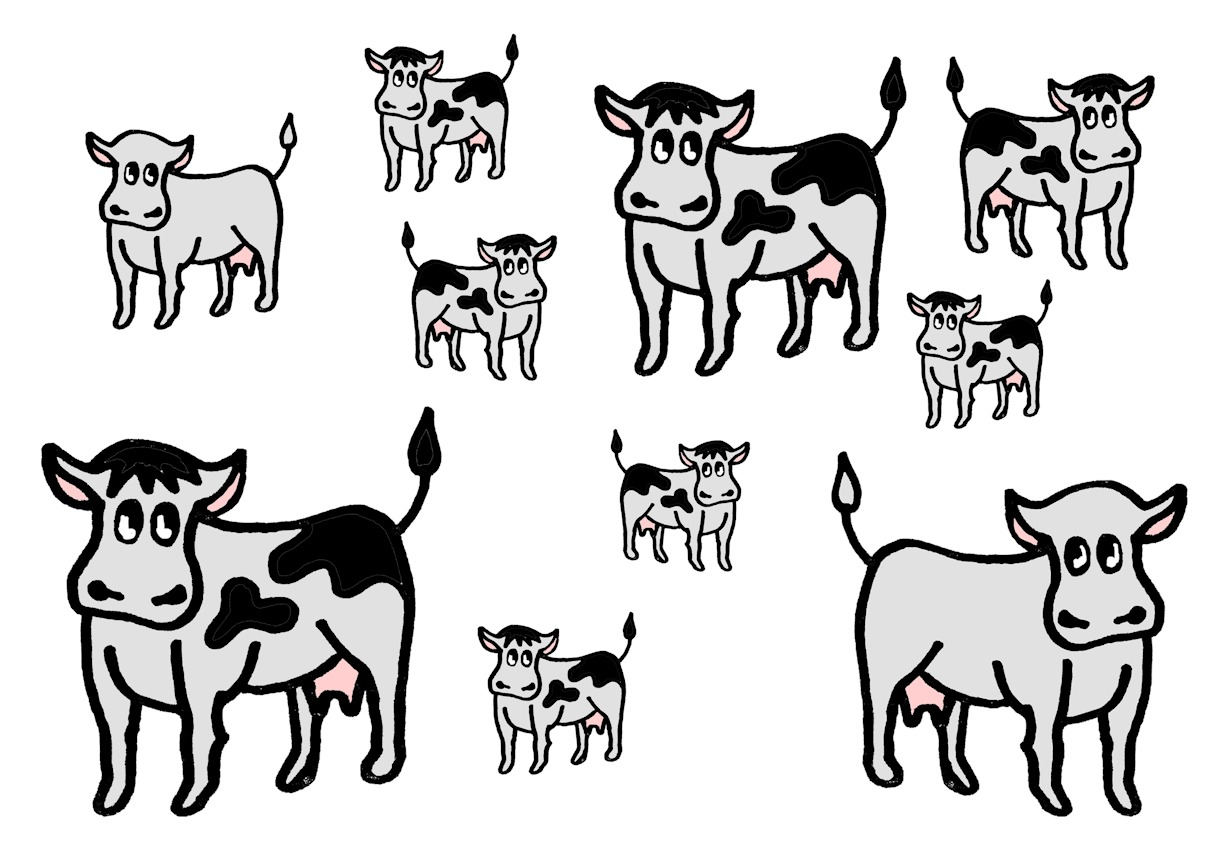
\includegraphics[scale=0.8]{Figure1.jpg}
    \caption{`not all' reading of \REF{kis-zet:nehany tehen}}
    \label{kis-zet:cow not all}
\end{minipage}
\begin{minipage}[b]{0.49\textwidth}
    \centering
    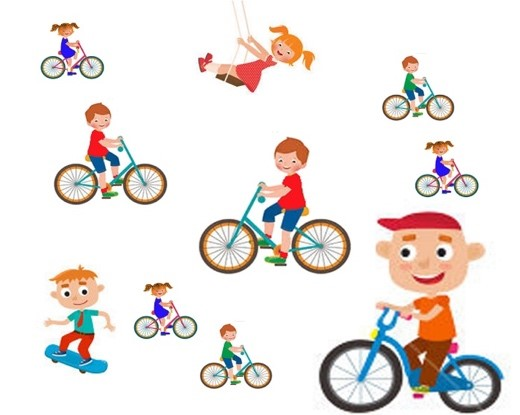
\includegraphics[scale=0.8]{Figure3.jpg}
    \caption{`not all' reading of \REF{kis-zet:nehany gyerek}}
    \label{kis-zet:bicycle not all}
\end{minipage}
~
\begin{minipage}[b]{0.49\textwidth}
    \centering
    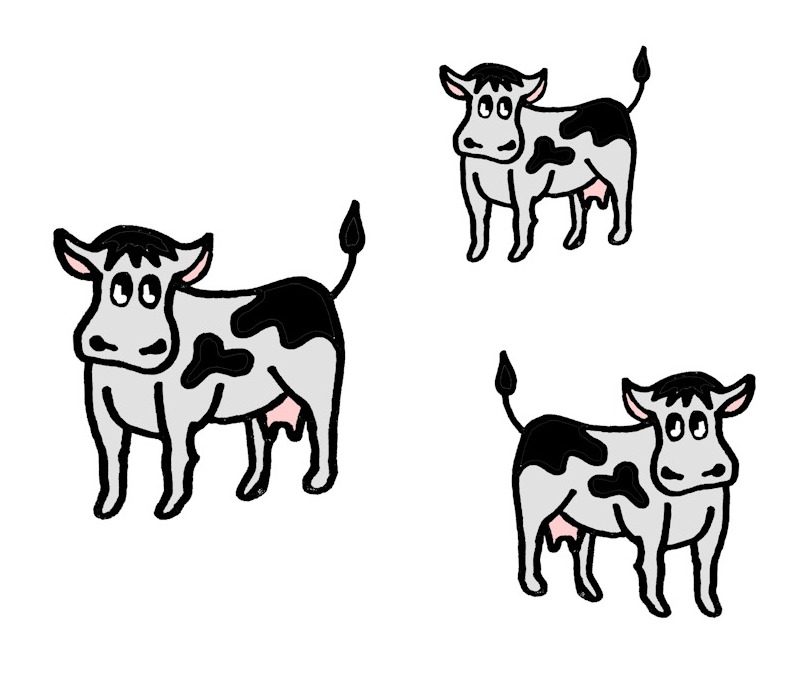
\includegraphics[scale=0.8]{Figure2.jpg}
    \caption{`a few' reading of \REF{kis-zet:nehany tehen}}
    \label{kis-zet:com few}
\end{minipage}
\begin{minipage}[b]{0.49\textwidth}
    \centering
    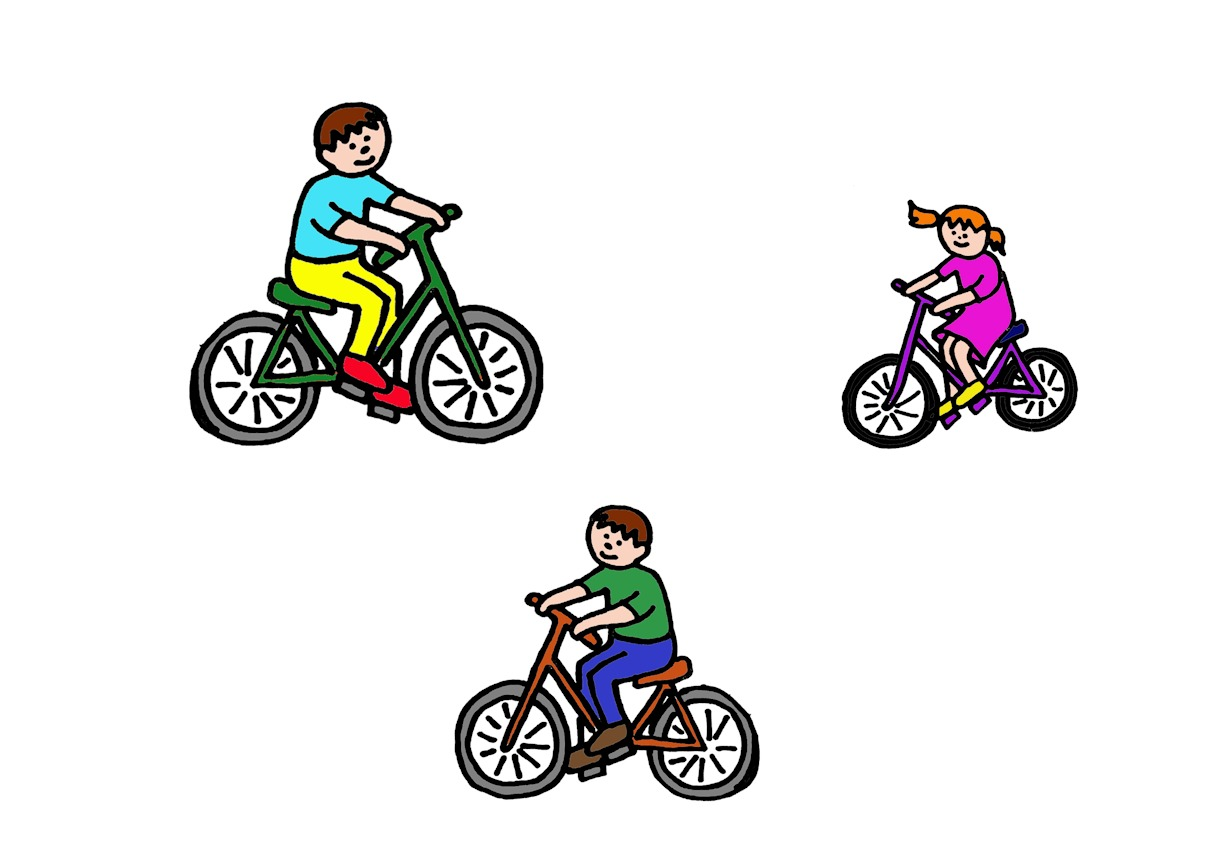
\includegraphics[scale=0.8]{Figure4.jpg}
    \caption{`a few' reading of \REF{kis-zet:nehany gyerek}}
    \label{kis-zet:bicycle few}
\end{minipage}
\end{figure}

The filler stimuli involved quantifiers other than `some', among them \textit{minden} `every', \textit{csak négy} `only four', \textit{ötnél több} `more than five'.

\subsubsection{Procedure}

The children were tested individually by the experimenter and a helper in a quiet room at their school. The pairs of pictures appeared on a computer screen, and they were accompanied by a sentence allegedly uttered by a puppet, recorded in advance. The child had to tell which of the two pictures the puppet was talking about. The child’s answers were recorded both on paper, and by a video camera.

\subsubsection{Results} 

Responses were encoded as binary data, 1 for `a few', 0 for the `not all' interpretation of \textit{néhány}. The mean responses of the age groups are shown in \figref{kis-zet:exp1 results}. 

\begin{figure}
    \centering
    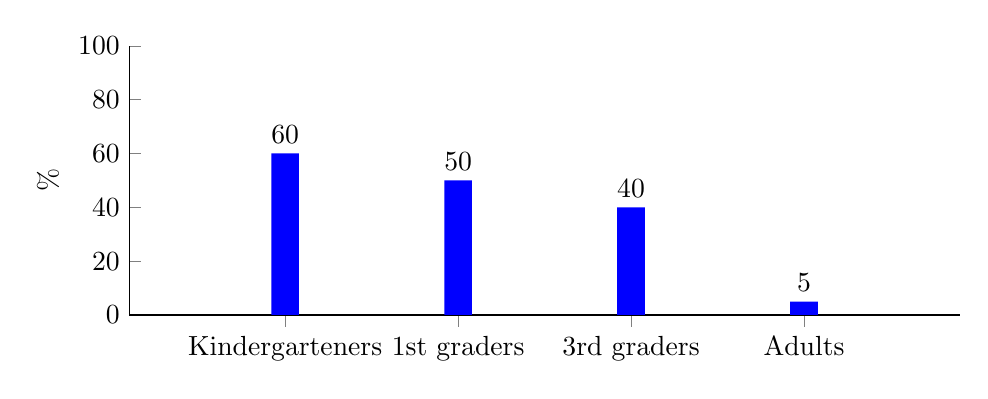
\begin{tikzpicture}
    \begin{axis}[
% 	xlabel={Level of \textsc{uniq/max}},  
	ylabel={\%}, 
    % ylabel={a,b},
    	nodes near coords, 
    % 	nodes near coords style={text=black},
        nodes near coords align={vertical},
	axis lines*=left, 
        width  = \textwidth,
	height = 5cm,
	ymin=0,
	ymax=100,
	ytick distance=20,
	xtick=data,
	ylabel near ticks,
% 	x tick label style={font=\sffamily},
	ybar,
	enlarge x limits=0.3,
	symbolic x coords={Kindergarteners, 1st graders, 3rd graders, Adults},
    % symbolic x coords={a,b},
	]
	\addplot[fill=blue,draw=none] coordinates {
	    (Kindergarteners,60)
        (1st graders,50)
        (3rd graders,40)
        (Adults,5)
	}; 
    \end{axis}
    \end{tikzpicture}
    \caption{The proportion of `a few' choices in Experiment 1}
    \label{kis-zet:exp1 results}
\end{figure}

% \begin{figure}
%     \centering
%     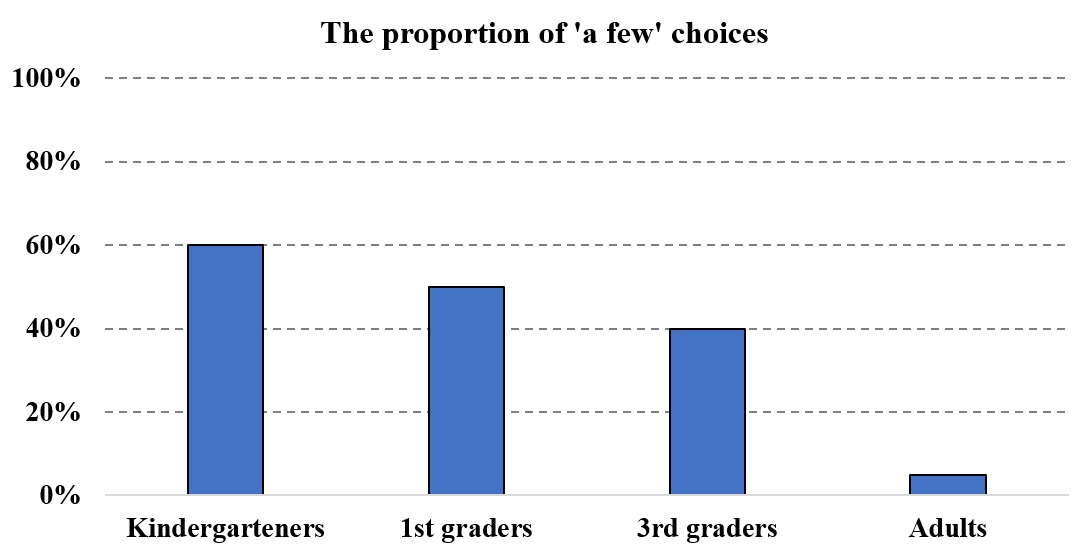
\includegraphics[scale=0.6]{Figure5.jpg}
%     \caption{`a few' choices in Experiment 1}
%     \label{kis-zet:exp1 results}
% \end{figure}

Binomial generalised mixed-effect models with random intercepts were run, with response as the dependent variable, group as the fixed effect, and participant and item as random effects. Calculations were carried out in R (\citealt{rcore19}), using glmer() from the lme4 package \citep{bates2015fitting} and Anova() from the car package \citep{fox2018r} for the calculation of simulated $p$-values.

The effect of the group was highly significant ($\chi^{2}(3) = 25.356, p < 0.001$). Pairwise comparisons of the age groups revealed that the response patterns of adults differed significantly from those of kindergarteners ($z = 4.949, p < 0.001$), 1$^\text{st}$ graders ($z = 4.211, p < 0.001$), and 3$^\text{rd}$ graders ($z = 3.579, p < 0.001$), whereas that there was no significant difference among the performance of the three groups of children (all three $z > -1.897, p > 0.058$).    

\subsubsection{Discussion} 

Our experiment aimed to test how young children interpret \textit{néhány} `some' NPs. Our hypothesis is that \textit{some}, and its Hungarian equivalent \textit{néhány} have a partitive and a non-partitive reading. For adults, the interaction of the structural position, the prosody, the internal structure of the `some'-phrase, and the selectional properties of the predicate usually support one of the readings and blocks the other one. For young children, however, the cognitively simpler non-partitive reading may be more easily accessible in all conditions than the partitive reading requiring the identification of two discourse referents (the set denoted by the quantified phrase, and a superset).	Our experiment tested this hypothesis by a forced choice test, where subjects listened to sentences involving a topicalized, hence partitive, \textit{néhány} `some' phrase, and they were offered both the `not all' and the `a few' readings. The results confirmed that for adults, \textit{néhány} occurring in a topicalized phrase clearly means `not all'. For six-year-olds, on the contrary, the `a few' reading is primary; it was chosen significantly more times than the `not all' interpretation. 

Although the mean results of all three age groups were relatively close to 50\%, the great majority of children were apparently not guessing but followed clear strategies. The proportion of those giving very consistent answers, choosing the same type of interpretation in 5 or 6 cases out of 6 was 83\% among the kindergarteners, 75\% among the first graders, and 65\% among the 3rd graders. The proportion of the children consistently opting for the `a few' interpretation, and the proportion of those consistently choosing the `not all' reading changed from age group to age group as shown in \tabref{kis-zet:table:1}.

\begin{table}
\centering
\begin{tabular}{c c c c c} 
\lsptoprule
 {} & Kindergarteners & 1$^\text{st}$ graders & 3$^\text{rd}$ graders & Adults \\
\midrule
`a few' & $54\%$ & $35\%$ & $25\%$ & $0\%$ \\
`not all' & $29\%$ & $40\%$ & $40\%$ & $88\%$ \\
\lspbottomrule
\end{tabular}
\caption{Proportions of children giving consistent answers (5 or 6 identical choices out of 6)}
\label{kis-zet:table:1}
\end{table}

In the older groups of children, both the proportion of the inconsistent answers and the proportion of consistent `not all' choices was higher, which supports the hypothesis that the `a few' reading appears first, and the partitive `not all' reading emerges – and the ambiguity of \textit{néhány} solidifies – with some delay. 

The fact that children show a clear preference for the `a few' interpretation around the age of six and for the `not all' interpretation around the age of nine provides evidence against the view that their choices are based on the reading `some and possibly all', the so-called logical meaning of \textit{néhány/some}. This meaning is compatible with both members of the picture pairs, hence if the children had relied on the meaning `some and possibly all', their choices would have been random. 

The relevant distinction that children become sensitive to around the age of nine is the [$\pm$partitive] feature attributable to `some'. It is the recognition of the [$+$partitive] feature of topics that opens the way to realizing that `some' and `all' are scale members, and the use of `some' implicates the falsehood of `all'.

\subsection{Experiment 2: A truth value judgement task}

Experiment 1 served to identify children's default interpretation of topicalized \textit{néhány} phrases; however, it left open the question whether the reading chosen by the children is the only accessible reading or the preferred reading for them. So as to answer this question, we carried out a second experiment. Experiment 2 also aimed to clarify whether children's interpretation of a \textit{néhány} phrase is affected by its structural position and prosody, more precisely, by the [$\pm$partitive] feature associated with that position and stress pattern. 

\subsubsection{Participants}

The children participating in Experiment 2 were the same as those participating in Experiment 1. We also tested an adult control group of 16 adults.

\subsubsection{Materials and methods}

The children had to judge the truth value of 23 sentence–picture pairs, 12 test cases and 11 fillers. The test sentences involved a \textit{néhány} phrase in $2\times 2$ conditions. The factors the effect of which we tested were (i) topic position (in SpecTopP, preceding the pitch accent), associated with a [$+$partitive] feature, versus non-topic position (in SpecPredP, bearing a pitch accent), associated with a [$-$partitive] feature in adult Hungarian, and (ii) `a few' versus `not all' reading shown in the visual stimulus. These factors yielded the following four conditions (C1--C4):

\begin{description}
\item[C1:] [$+$topic] \textit{néhány} NP, `not all' reading, e.g.:

\ea
\gll \label{kis-zet:szamar} [$_\text{TopP}$ 	Néhány 	szamár 	[$_\text{PredP}$ 	szürke.]]\\  
     {} {} some donkey {} grey\\ 
\glt `Some donkeys are grey.'
\z

% \begin{figure}[h!]
%    \centering
%    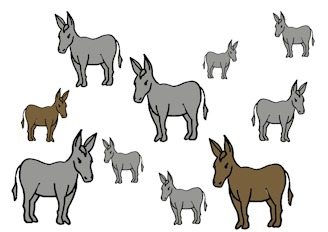
\includegraphics[scale=0.62]{Figure6.jpg}
%    \caption{Picture accompanying example \REF{kis-zet:szamar}}
%    \label{kis-zet:c1}
% \end{figure}

\item[C2:] [$+$topic] \textit{néhány} NP, `a few' reading, e.g.:

\ea
\gll \label{kis-zet:ceruza} [$_\text{TopP}$ 	Néhány ceruza 	[$_\text{PredP}$ 	ki 		van 	hegyezve.]]\\  
    {} {} some pencil {} out is sharpened\\ 
\glt `Some pencils have been sharpened.'
\z

% \begin{figure}[h!]
%    \centering
%    
\includegraphics[scale=0.15]{Figure7a.jpg}
%    \caption{Picture accompanying example \REF{kis-zet:ceruza}}
%    \label{kis-zet:c2}
% \end{figure}


\item[C3:] [$-$topic] \textit{néhány} NP, `a few' reading, e.g.:
\ea
\gll \label{kis-zet:barack}[$_\text{PredP}$ Néhány barack nő az ág-on.]\\ {} some apricot grows the branch-on\\ 
\glt `Some apricots are growing on the branch.'
\z

% \begin{figure}[h!]
%    \centering
%    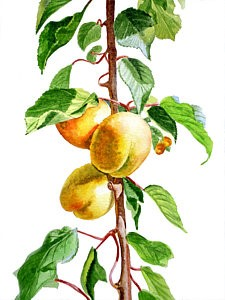
\includegraphics[scale=0.6]{Figure8.jpg}
%    \caption{Picture accompanying example \REF{kis-zet:barack}}
%    \label{kis-zet:c3}
% \end{figure}


\item[C4:] [$-$topic] \textit{néhány} NP, `not all' reading, e.g.:

\ea
\gll \label{kis-zet:alma}[$_\text{PredP}$ Néhány alma van a kosár-ban.]\\ 
{} some apple is the basket-in\\ 
\glt ‘There are some apples in the basket.’
\z

% \begin{figure}[h!]
%    \centering
%    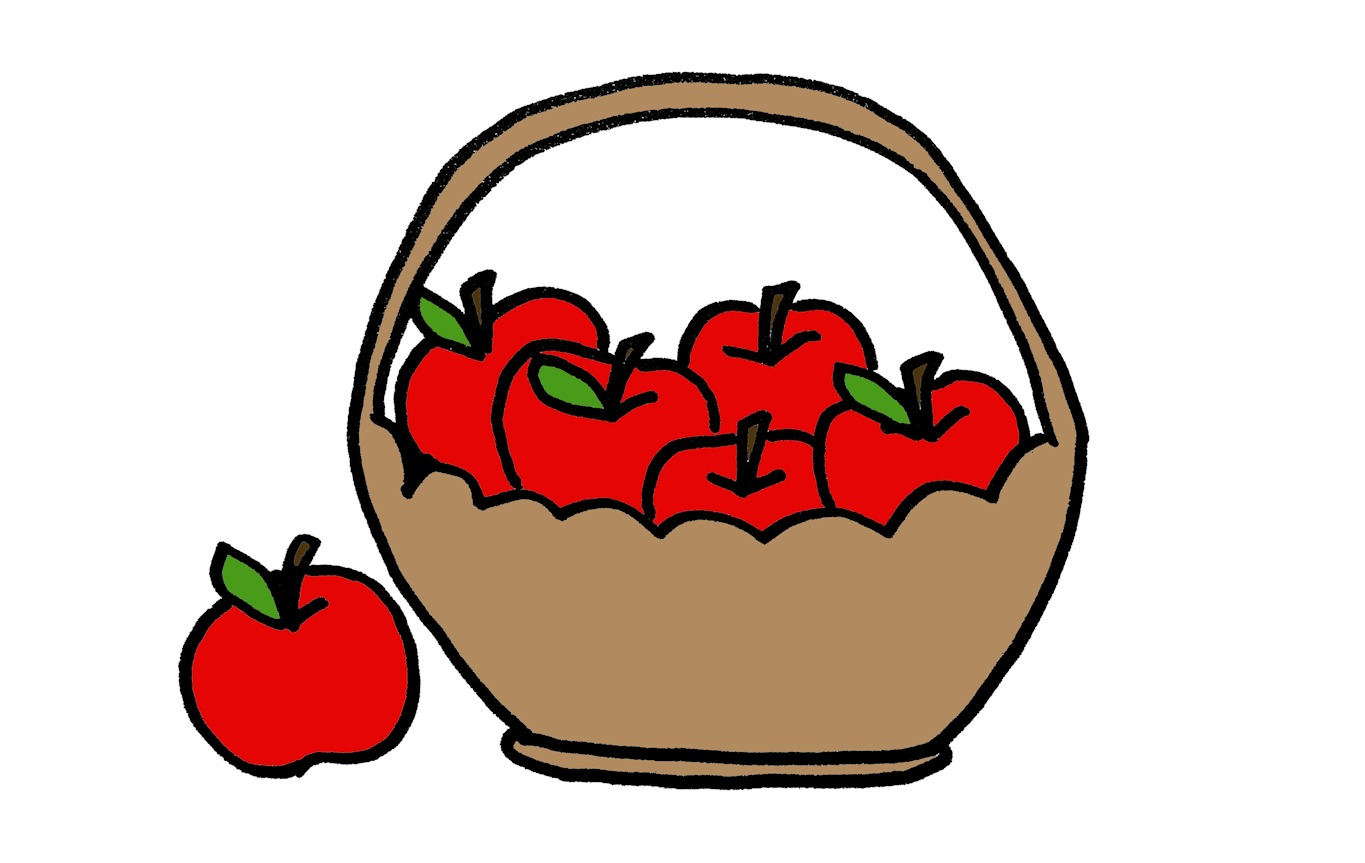
\includegraphics[scale=0.18]{Figure9.jpg}
%    \caption{Picture accompanying example \REF{kis-zet:alma}}
%    \label{kis-zet:c4}
% \end{figure}

\end{description}

\begin{figure}[h]
\RawFloats
\centering
\begin{minipage}[b]{0.49\textwidth}
    \centering
    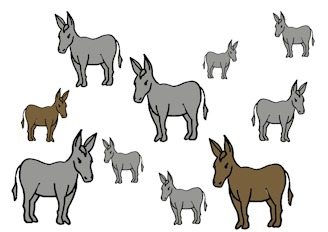
\includegraphics[scale=0.62]{Figure6.jpg}
    \caption{Picture accompanying \REF{kis-zet:szamar}}
    \label{kis-zet:c1}
\end{minipage}
\begin{minipage}[b]{0.49\textwidth}
    \centering
    
\includegraphics[scale=0.15]{Figure7a.jpg}
    \caption{Picture accompanying \REF{kis-zet:ceruza}}
    \label{kis-zet:c2}
\end{minipage}
~
\begin{minipage}[b]{0.49\textwidth}
    \centering
    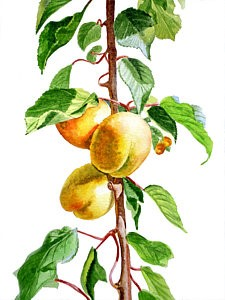
\includegraphics[scale=0.6]{Figure8.jpg}
    \caption{Picture accompanying \REF{kis-zet:barack}}
    \label{kis-zet:c3}
\end{minipage}
\begin{minipage}[b]{0.49\textwidth}
    \centering
    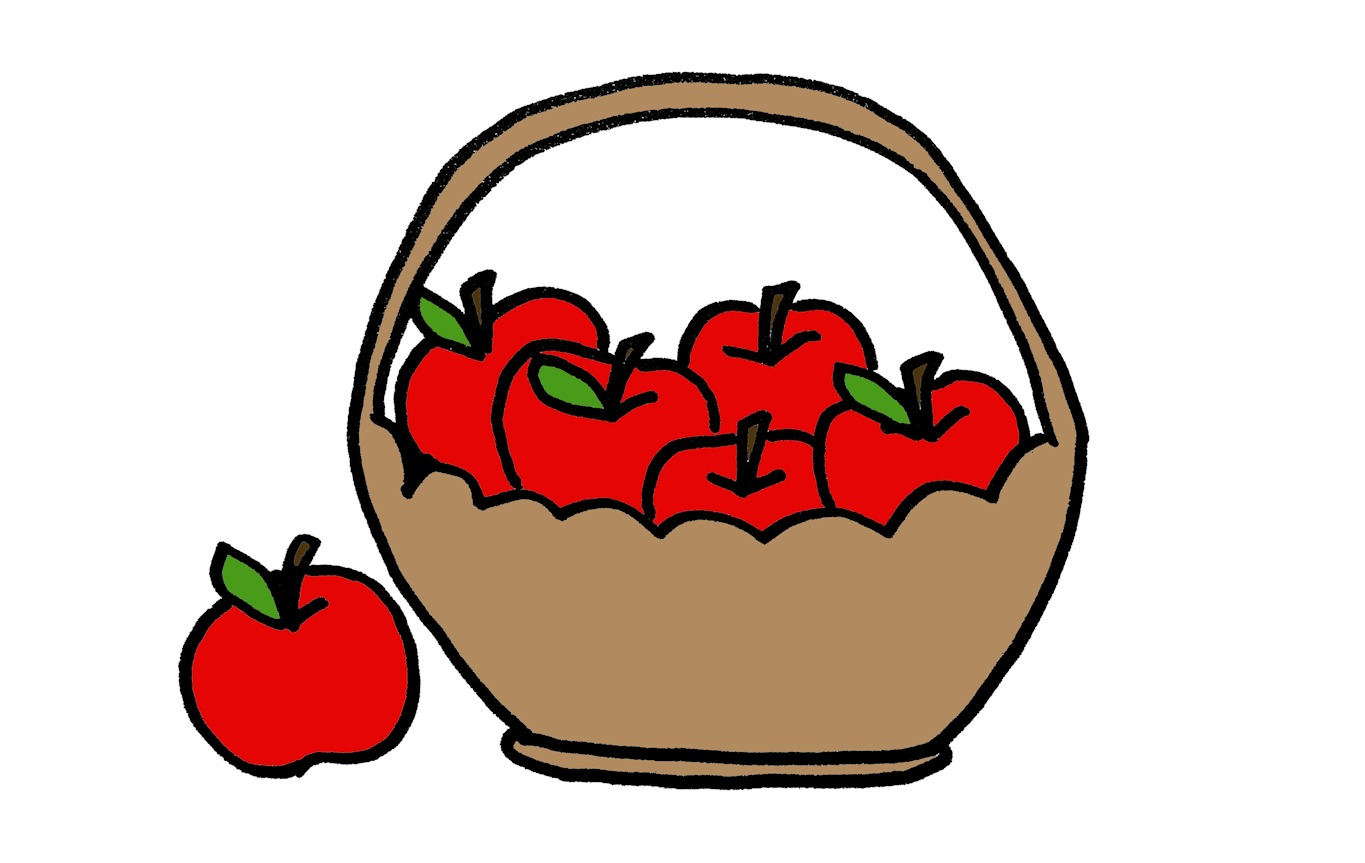
\includegraphics[scale=0.18]{Figure9.jpg}
    \caption{Picture accompanying \REF{kis-zet:alma}}
    \label{kis-zet:c4}
\end{minipage}
\end{figure}

Each condition was represented by 3 examples. The fillers were sentence involving quantifiers such as  \textit{minden} `every',  \textit{legtöbb} `most',  \textit{legalább három} `at least three', \textit{csak négy} `only four', etc.

\subsubsection{Procedure}

Experiment 2 was carried out in the same session as Experiment 1. The pictures were presented to each child on a computer screen one by one, together with the corresponding sentence allegedly uttered by a puppet, recorded in advance. The child was told that the puppet explaining what she saw in each picture did not have her glasses on, hence she did not always see the picture properly. The child had to judge whether the puppet said correctly what the picture showed. The child’s answers were recorded both on paper, and by video camera.

\subsubsection{Results}

The sentences were found to be true in the great majority of cases in all conditions.  The proportions of yes answers in the four conditions are shown in \tabref{kis-zet:table:2}.

\begin{table}
\centering
\begin{tabular}{l l l l l}
\lsptoprule
{} & C1:[$+$topic] & C2:[$+$topic] & C3:[$-$topic]  & C4:[$-$topic] \\
{} & `not all' & `a few' & `a few' & `not all' \\
\midrule
Kindergarteners & 78\% & 82\% & 83\% & 65\% \\
1$^\text{st}$ graders & 80\% & 70\% & 82\% & 77\% \\
3$^\text{rd}$ graders & 80\% & 62\% & 77\% & 77\% \\
\midrule
All children: & 79\% & 71\% & 81\% & 73\% \\
Adults:	 & 69\% & 49\% & 98\% & 55\% \\
\lspbottomrule
\end{tabular}
\caption{Acceptance rates of sentences with a \textit{néhány} phrase in the four conditions}
\label{kis-zet:table:2}
\end{table}

Responses were encoded as binary data, 1 for `true', 0 for `false'. Binomial generalised mixed-effect models with random intercepts were run, with response as the dependent variable, the interaction of structural position ([$+$topic] versus [$-$topic]) and picture type (`a few' versus `not all'), as well as group as fixed effects, with participant and item as random effects. Calculations were carried out in R \citep{rcore19}, using glmer() from the lme4 package \citep{bates2015fitting} and Anova() from the car package \citep{fox2018r} for the calculation of simulated $p$-values.

While age group did not have a significant effect on the response patterns (all three $z > 1.350, p > 0.126$), the effects of sentence type ($z = -2.821, p = 0.005$), picture type ($z = -2.528, p = 0.011$) and the interaction of sentence type and picture type ($z = 2.710, p = 0.007$) were all significant. In the case of `a few' pictures, the acceptance rate of sentences with a topicalized \textit{néhány} phrase was lower, while that of sentences with a non-topical \textit{néhány} phrase was exceptionally high. When `not all' pictures were evaluated, the difference between the two sentence types was considerably smaller, but in this case, it was the sentence type with a topicalized \textit{néhány} phrase that was accepted more frequently. 

\subsubsection{Discussion}

Among the adults, the acceptance of non-topic \textit{néhány} phrases under the `a few' interpretation was practically unanimous. The acceptance of topicalized, hence partitive, \textit{néhány} phrases under the `not all' reading, however, was merely 69\%, lower than expected. Those rejecting some of the sentence-picture combinations, e.g. that in \REF{kis-zet:szamar}, explained that for them, the topicalized \textit{néhány} means `a relatively small subset of', i.e., it has both the `not all' and `a few' meaning components.  Example \REF{kis-zet:szamar} would be true of \figref{kis-zet:c1} if the subset of grey donkeys were smaller than the subset of brown donkeys. The acceptance of topicalized \textit{néhány} phrases coupled with a visual representation corresponding to the `a few' interpretation, as well as the acceptance of non-topic \textit{néhány} phrases coupled with a visual representation corresponding to the `not all' reading was stimulus dependent to a large extent; apparently, it depended on whether or not the participant could coerce the reading determined by the structural position of the \textit{néhány} NP. For example, the topicalized \textit{néhány ceruza} `some pencils' in \REF{kis-zet:ceruza} coupled with a picture showing a few pencils (\figref{kis-zet:c2}) was accepted by fewer participants than example \REF{kis-zet:nehany gyerek tanul} coupled with  \figref{kis-zet:children reading}. 

\ea
\gll \label{kis-zet:nehany gyerek tanul}[$_\text{TopP}$ Néhány gyerek [$_\text{PredP}$ tanul.]]\\ 
     {} some child {} studies\\ 
\glt `Some children are studying.'
\z

\begin{figure}
    \centering
    
\includegraphics[scale=0.7]{Figure10.jpg}
    \caption{Picture accompanying \REF{kis-zet:nehany gyerek tanul}}
%    \caption{Picture accompanying example \REF{kis-zet:nehany gyerek tanul}}
    \label{kis-zet:children reading}
\end{figure}

The adults accepting this sentence–picture combination explained that they can assume these children to represent the subset of a class where the rest of the children are not studying – i.e., they can coerce a partitive reading. In the case of a set of sharpened pencils it is harder to imagine the presence of a superset that is out of view. 

Similarly, the non-topic \textit{néhány} phrase in \REF{kis-zet:alma} under the ʻnot all’ reading in \figref{kis-zet:c4} was accepted by more adults than sentence \REF{kis-zet:piros ceruza} coupled with \figref{kis-zet:pencils} presumably because the apple near the basket can be considered to be outside the relevant domain of quantification more easily than the non-red pencils in the mug.\footnote{\citet{ekisszt18} present experimental evidence demonstrating the interaction of the visual representation of the domain of quantification and children’s ability to carry out scalar implicature.} 

\ea\label{kis-zet:piros ceruza}
\gll [$_\text{PredP}$ Néhány piros ceruza van a bögré-ben.]\\  
    {} some red pencil is the mug-in \\ 
\glt ‘There are some red pencils in the mug.’
\z


\begin{figure}
    \centering
    
\includegraphics[scale=0.6]{Figure11.jpg}
    \caption{Picture accompanying \REF{kis-zet:piros ceruza}}
%    \caption{Picture accompanying example \REF{kis-zet:piros ceruza}}
    \label{kis-zet:pencils}
\end{figure}

The children, too, found non-topic \textit{néhány} phrases under the `a few' interpretation (C3) and topicalized \textit{néhány} phrases under the `not all' reading (C1) the most acceptable. Crucially, however, they also accepted both 71\% of the topicalized \textit{néhány} NPs with the ʻa few’ reading, and 73\% of the non-topic \textit{néhány} NPs with a `not all' reading, and these acceptance rates are significantly different from the 49--55\% acceptance rates of the adults. Whereas adults assign the `a few' reading to non-topic \textit{néhány} phrases,
and tend to assign the `not all' interpretation to topicalized \textit{néhány}
phrases, for kindergarteners and 1st graders, there is no significant difference between the acceptability of \textit{néhány} phrases in the four conditions. We attested a significantly higher acceptance of the `a few' reading in [$-$topic] contexts than in [$+$topic] contexts only among the 3rd graders. In the case of younger children, there is no significant correlation between the structural and prosodic conditions determining the partitivity feature of the \textit{néhány} phrase and the interpretation they assign to it. 

\section{Conclusion}\label{kis-zet:sec:conclusion}

A series of previous experiments \citep[e.g.][]{noveck2001children,papafragou2003scalar,miller2005young,papafragouskordos16,pouscoulous2007developmental} found that children tend to accept sentences with a topical subject represented by a \textit{some} NP (or its Greek, French etc. equivalent), e.g., \textit{Some (of the) donkeys are grey}, in situations where the predicate holds of all the subject referents, i.e., where all the donkeys are grey. Our experiments carried out with Hungarian children have yielded similar results. Adults are believed to interpret such sentences based on Grice's Maxim of Quantity, assuming that the speaker has been as informative as possible. A situation where all the donkeys are grey could have been truthfully described by the sentence \textit{All (of the) donkeys are grey}, hence the speaker's use of \textit{some} indicates that s/he had reasons not to use a stronger term, e.g. \textit{all}. Therefore, \textit{Some (of the) donkeys are grey} gives rise to the scalar implicature that not all donkeys are grey. Children's failure to carry out such implicatures was initially attributed to their pragmatic inexperience; it was claimed that for them, pragmatics does not overwrite logic \citep{noveck2001children}. This explanation, however, cannot account for the fact that children have much less difficulty with scalar implicatures involving definite numbers \citep[cf. e.g.,][]{papafragou2003scalar,ekisszt18}. In Experiment 1 of \citet{papafragou2003scalar}, children’s success rate with a scalar implicature involving the numbers \textit{two} and \textit{three} was 65\%, whereas their success rate with a scalar implicature involving \textit{some} and \textit{all} was merely 12.5\%. In their Experiment 2, which involved some training and some contextual manipulations, the success rate of scalar implicatures rose to 90\% in the case of \textit{two} and \textit{three}; however, it rose only to 52.5\% in the case of \textit{some} and \textit{all}. These facts indicate that the particular way children relate \textit{some} and \textit{all} also involves a factor other than their ability to derive scalar implicatures.

The alternatives-based theory of \citet{barner2011accessing} claims that children’s difficulties with scalar implicature in the case of specific scales are due to a failure to generate relevant alternatives for the given scale. Thus, although children may know already at the age of two that \textit{some} and \textit{all} denote different set relations, they do not know that they are members of the same scale. The hypothesis we tested shares an element of this claim: in our view, children do not realize that \textit{some} and \textit{all} are scale mates because they identify \textit{some} with its non-partitive variant, which forms a scale with the non-partitive \textit{many}. 

The starting point of our explanation of children’s interpretation of `some' was that `some' is inherently ambiguous; it has a [$+$partitive] meaning corresponding to `not all', and a [$-$partitive] meaning corresponding to `a few'. For adults, the structural position, the prosody, the internal structure of the `some'-phrase, and/or the selectional properties of the predicate determine the partitivity of the `some'-phrase in most cases; for instance, the subject-topic `some'-phrases of the test sentences of former experiments are clearly [$+$partitive]. Young children, however, are not sensitive to the partitivity feature arising in various contexts, or they are not aware of its significance in the interpretation of `some'. Children presumably acquire the easier, non-partitive reading first, and tend to overgeneralize it for a while. For English adults, the genitive construction in cases like \textit{some of the donkeys are grey} would strongly suggest that the grey donkeys represent a proper subset of a relevant set of donkeys. However, \textit{all of the donkeys} means the same as \textit{all donkeys}, \textit{each of the donkeys} means the same as \textit{each donkey}, \textit{which of the donkeys} means the same as \textit{which donkey}, so it may not be obvious for children that the interpretation of \textit{some of the donkeys} may be different from the interpretation of \textit{some donkeys}.

We tested these assumptions with two experiments. The first experiment, a forced choice sentence-picture matching task, showed that six-year old Hungarian children significantly more often assign the `a few' reading than the `not all' reading to topicalized \textit{néhány} NPs. Furthermore, the proportion of children who consistently (5 or 6 times out of 6) select the `a few' reading is 54\% among the six-year-olds, and is still 35\% among the seven-and-half-year-olds, and 25\% among the nine-and-half-year-olds. These results are in accord with the assumption that the reading that is first associated with `some' by young children and which remains the default reading for them for some time is the non-partitive `a few' interpretation. 

The second experiment, a truth value judgement task aimed to clarify whether the `a few' reading of \textit{néhány} is the only reading for the majority of children, or it is merely its primary interpretation. We tested whether children can access both readings of \textit{néhány}, and whether they are aware of the correlation between the structural position and prosody, and the interpretation of the \textit{néhány} NP. It has turned out that children also accept the `not all' interpretation of `some', and the acceptance rate of both the `a few' and the `not all' readings is roughly the same irrespective of the partitivity feature of the `some' NP in the given context. The acceptance of the `not all' interpretation is not significantly higher in the case of topicalized \textit{néhány} phrases than in the case of non-topic \textit{néhány} phrases.

The two findings: children's initial bias towards the `a few' interpretation of `some', and their insensitivity to the partitivity feature of the `some' NP can explain children's non-adult-like behaviour with respect to `some' NPs. They accept the sentence `Some (of) the donkeys are grey' in a situation where all of the donkeys are grey because `some' means for them `a relatively small number', or `a non-empty set', i.e., they interpret the sentence as `a relatively small number of donkeys are grey'. They realize that `some' and `all' can be scale members, and the use of `some' can implicate the infelicity of `all' only when, around the age of nine, they become aware of the partitivity of `some'-phrases in topic position and in some other specific contexts. 


\section*{Abbreviations}

\begin{tabularx}{.5\textwidth}{@{}lX@{}}
\textsc{1}&{first person}\\
\textsc{3}&{third person}\\
\textsc{acc}&{accusative}\\
\end{tabularx}%
\begin{tabularx}{.5\textwidth}{@{}lX@{}}
\textsc{past}&{past tense}\\
\textsc{prt}&{particle}\\
\textsc{sg}&{singular}\\
\end{tabularx}

\section*{Acknowledgements}
We owe thanks to the Hungarian National Research Fund of the National Research, Development and Innovation Office for the support of grants K 108951 and KH 130558, as well as to Bükköny Kindergarten and Farkasréti Primary School of District 11, Budapest.

{\sloppy\printbibliography[heading=subbibliography,notkeyword=this]}

\end{document}
